%
% Heap and Stack organization -- traditional.
%
\documentclass[border=3mm]{standalone}
\usepackage{tikz}
\usetikzlibrary{circuits.ee.IEC}

\begin{document}

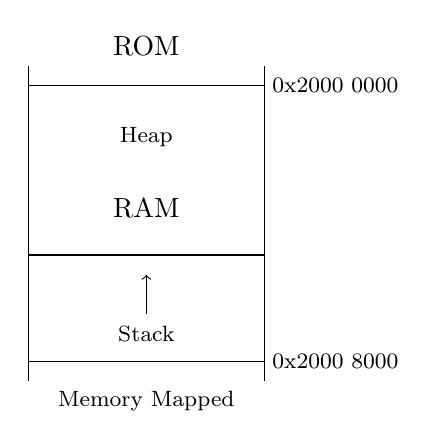
\begin{tikzpicture}
    \draw [-] (0,0) to (0,4);
    \draw [-] (3,0) to (3,4);
    \draw [-] (0,0.25) to (3,0.25);
    \draw [-] (0,3.75) to (3,3.75);
    \draw [-] (0,1.60) to (3,1.60);
    \draw [<-] (1.50,1.35) to (1.50,0.85);
    \node (ram_start) at (3.1,3.75) {};
    \node (ram_end) at (3.1,0.25) {};
    \node (rom) at (1.50,4.25) {ROM};
    \node (ram) at (1.50,2.20) {RAM};
    \node (heap) [font=\footnotesize] at (1.50,3.10) {Heap};
    \node (stack) [font=\footnotesize] at (1.50,0.60) {Stack};
    \node (stack) [font=\footnotesize] at (1.50,-0.25) {Memory Mapped};
    \node [font=\footnotesize,right] at (ram_start.west) {0x2000 0000};
    \node [font=\footnotesize,right] at (ram_end.west) {0x2000 8000};
\end{tikzpicture}

\end{document}

